\documentclass[11pt]{article}
\usepackage[utf8]{inputenc}
\usepackage{graphicx}
\usepackage{grffile} % robust graphics paths with spaces/parentheses
\usepackage{float}
\usepackage{hyperref}
\usepackage{geometry}
\usepackage{booktabs}
\usepackage{subcaption}
\usepackage{xcolor}
\usepackage{fancyhdr}
\usepackage{titlesec}
\usepackage{enumitem}
\usepackage{amsmath}
\usepackage{microtype}

\geometry{margin=1in, top=1.2in, bottom=1.2in}

% Image search paths (handles directories with spaces)
\graphicspath{{../JupyterOutputs/}{../JupyterOutputs/Classification (Final)/}{../JupyterOutputs/Classification (Tuning)/}{../JupyterOutputs/VisualizationPreprocessing/}{../JupyterOutputs/PatternAnalysis/Diagnostics/}}

% Header and footer
\pagestyle{fancy}
\fancyhf{}
\fancyhead[L]{Crime Analyzer}
\fancyhead[R]{User Guide}
\fancyfoot[C]{\thepage}

% Section formatting
\titleformat{\section}{\Large\bfseries\color{black}}{\thesection}{1em}{}
\titleformat{\subsection}{\large\bfseries}{\thesubsection}{1em}{}

% Hyperlink setup
\hypersetup{
    colorlinks=true,
    linkcolor=black,
    filecolor=magenta,
    urlcolor=cyan,
    citecolor=green!50!black
}

\title{\Huge\textbf{Crime Analyzer}\\
       \Large\textit{User Guide for Tourist Safety Application}}
\author{Ferdinando Muraca, Carlo Vincenzo Stanzione}
\date{\today}

\begin{document}

\maketitle
\tableofcontents
\newpage

\section{Executive Summary}

\subsection{System Overview}
The Crime Analyzer is a machine learning solution that assesses criminal risk for tourists in New York City. Using historical NYPD complaint data and advanced spatio-temporal modeling, the system provides binary risk classifications (HIGH\_RISK/LOW\_RISK) with confidence scores and explainable predictions.

\subsection{Key Capabilities}
\begin{itemize}[leftmargin=*]
\item Real-time safety assessment based on location, time, and user demographics
\item Explainable predictions with feature attribution
\item 96.49\% overall accuracy with specialized handling of high-risk scenarios
\item Pattern analysis revealing crime trends and associations
\end{itemize}

\subsection{Target Users}
\begin{itemize}[leftmargin=*]
\item \textbf{Tourists:} Personal safety assessment and risk awareness
\item \textbf{City Planners:} Evidence-based resource allocation and urban development
\item \textbf{Law Enforcement:} Predictive insights for patrol optimization
\end{itemize}

\section{Quick Start Guide}

\subsection{Getting Started in 3 Steps}
\begin{enumerate}
\item \textbf{Provide Your Information}
  \begin{itemize}
  \item Allow location access (GPS coordinates)
  \item Enter basic demographics (age group, sex, race; categories follow NYPD definitions)
  \item System automatically detects current time
  \end{itemize}

\item \textbf{Receive Your Assessment}
  \begin{itemize}
  \item Get immediate HIGH\_RISK or LOW\_RISK classification
  \item Review confidence score (higher = more certain)
  \item Read explanation of key risk factors
  \end{itemize}

\item \textbf{Make Informed Decisions}
  \begin{itemize}
  \item Use results as one factor in your safety planning
  \item Pay attention to low-confidence predictions (40-60\%)
  \item Consider local crime patterns provided with your result
  \end{itemize}
\end{enumerate}

\subsection{Interpreting Your Result}
\begin{itemize}[leftmargin=*]
\item \textbf{LOW\_RISK:} Favourable conditions based on historical patterns. Continue to apply common safety practices.
\item \textbf{HIGH\_RISK:} Elevated risk indicators were detected. Prefer well-lit, populated areas and consider adjusting timing/routes.
\item \textbf{Confidence:} Treat probabilities close to the 0.64 threshold as \textit{uncertain}. Use added caution or seek more context.
\item \textbf{Context Matters:} Review the surfaced trends to understand which factors (time, location, surroundings) are driving risk.
\item \textbf{Not a Guarantee:} Outcomes are probabilistic. For emergencies in NYC call \textbf{911}. This tool complements, not replaces, local advice.
\end{itemize}

\subsection{Example Usage Scenario}
\textbf{Scenario:} A tourist is planning their evening activities and wants to assess the risk of visiting Times Square around 9 PM.
\begin{itemize}[leftmargin=*]
    \item \textbf{Input:} They provide their location (Times Square coordinates), the current time (9 PM), and basic demographic data.
    \item \textbf{Assessment:} The system returns a \texttt{HIGH\_RISK} classification with a confidence score of 71\%.
    \item \textbf{Explanation:} The key contributing factors are the late hour (\texttt{hour\_21}) and the high density of bars in the area (\texttt{poi\_density\_bar}).
    \item \textbf{Context:} The system also shows relevant crime trends for Manhattan, such as a strong association between the "25-44" age group and male suspects.
    \item \textbf{Decision:} The tourist, now more aware of the specific risk factors, decides to remain in more crowded and well-lit areas.
\end{itemize}
\noindent The model's overall performance metrics, such as 96.49\% accuracy and a 90.47\% ROC-AUC score, provide confidence in this assessment. See Section \ref{sec:performance} for a complete evaluation.

\section{System Architecture and Technical Specifications}

\subsection{System Overview}
The Crime Analyzer implements a comprehensive machine learning pipeline designed for real-time crime risk assessment. The architecture follows enterprise-grade standards with modular components, comprehensive logging, and production-ready artifacts.

\subsubsection{Core Components}
\begin{itemize}[leftmargin=*]
\item \textbf{Data Pipeline:} NYPD complaint data integration and feature engineering
\item \textbf{ML Pipeline:} Logistic regression with RobustScaler preprocessing
\item \textbf{Inference Engine:} Production model with embedded preprocessing
\item \textbf{Explainability Module:} SHAP-based feature attribution
\item \textbf{Pattern Analysis:} FP-Growth frequent itemset mining
\end{itemize}

\subsection{Input Specification}
The system accepts structured input with the following required parameters:

\subsubsection{Required Inputs}
\begin{itemize}[leftmargin=*]
\item \textbf{Geographic Coordinates}
  \begin{itemize}
  \item Latitude: Decimal degrees [-90, 90]
  \item Longitude: Decimal degrees [-180, 180]
  \end{itemize}
\item \textbf{User Demographics}
  \begin{itemize}
  \item Age Group: Categorical (e.g., 25-44, 45-64)
  \item Race: Categorical (standardized NYPD categories).
  \item Sex: M/F (as recorded by NYPD categories).
  \end{itemize}
\end{itemize}

\subsubsection{Derived Features}
The system automatically generates 28 additional features from the input coordinates and timestamp:
\begin{itemize}[leftmargin=*]
\item \textbf{Temporal Features (10):} HOUR, DAY, WEEKDAY, IS\_WEEKEND, MONTH, YEAR, SEASON, TIME\_BUCKET, IS\_HOLIDAY, IS\_PAYDAY
\item \textbf{Geographic Features (2):} BORO\_NM, LOC\_OF\_OCCUR\_DESC
\item \textbf{POI-based Features (16):} Distance metrics and density scores for bars, nightclubs, ATMs, metros, schools, and bus stops
\end{itemize}

\subsection{Output Specification}
\begin{itemize}[leftmargin=*]
\item \textbf{Primary Output:} Binary classification \{HIGH\_RISK, LOW\_RISK\}
\item \textbf{Decision Threshold:} 0.64 (optimized for F1-score)
\item \textbf{Confidence Score:} Probability in [0,1] associated with the HIGH\_RISK class; returned as \texttt{confidence} alongside the label.
\item \textbf{Uncertainty Handling:} Low-confidence predictions (e.g., probabilities close to the decision threshold) should be surfaced to users/operators for cautious interpretation.
\item \textbf{Response Time:} $<$ 100ms (inference only, typical CPU)
\end{itemize}

\subsection{API Integration Design}
The system is architected for REST API deployment with the following endpoints:

\subsubsection{Prediction Endpoint}
\begin{verbatim}
POST /api/v1/predict
Content-Type: application/json

Request
{
  "latitude": 40.7580,
  "longitude": -73.9855,
  "timestamp": "2025-09-01T21:00:00Z",
  "age_group": "25-44",
  "race": "WHITE HISPANIC",
  "sex": "M"
}

Response
{
  "label": "HIGH_RISK",
  "confidence": 0.71,
  "threshold": 0.64,
  "explanations": {
    "top_features": [
      {"feature": "hour_21", "shap": 0.42},
      {"feature": "poi_density_bar", "shap": 0.18}
    ]
  },
  "trends": {
    "neighborhood": [
      {
        "context": "Borough:MANHATTAN",
        "antecedent": ["LOC_OF_OCCUR=INSIDE"],
        "consequent": ["HAS_POI=NO"],
        "support": 0.349,
        "confidence": 0.659,
        "lift": 1.031,
        "leverage": 0.011,
        "conviction": 1.059,
        "zhangs_metric": 0.0,
        "score": 0.356
      },
      { "context": "Borough:MANHATTAN", "antecedent": ["SUSP_AGE=25-44"], "consequent": ["SUSP_SEX=M"], "support": 0.236, "confidence": 0.780, "lift": 1.459, "leverage": 0.077, "conviction": 2.067, "zhangs_metric": 0.0, "score": 0.304 },
      { "context": "Borough:MANHATTAN", "antecedent": ["VIC_SEX=F"], "consequent": ["HAS_POI=NO"], "support": 0.319, "confidence": 0.799, "lift": 1.087, "leverage": 0.025, "conviction": 1.318, "zhangs_metric": 0.0, "score": 0.348 },
      { "context": "Borough:MANHATTAN", "antecedent": ["LAW_CAT=FELONY"], "consequent": ["HAS_POI=NO"], "support": 0.260, "confidence": 0.754, "lift": 1.025, "leverage": 0.006, "conviction": 1.074, "zhangs_metric": 0.0, "score": 0.283 },
      { "context": "Borough:MANHATTAN", "antecedent": ["TIME_BUCKET=EVENING"], "consequent": ["HAS_POI=NO"], "support": 0.245, "confidence": 0.746, "lift": 1.015, "leverage": 0.004, "conviction": 1.042, "zhangs_metric": 0.0, "score": 0.267 }
    ],
    "time_bucket": [
      {
        "context": "TimeBucket:EVENING",
        "antecedent": ["BORO=MANHATTAN"],
        "consequent": ["DIST_BIN=<250m"],
        "support": 0.197,
        "confidence": 0.818,
        "lift": 1.094,
        "leverage": 0.017,
        "conviction": 1.483,
        "zhangs_metric": 0.0,
        "score": 0.256
      },
      { "context": "TimeBucket:EVENING", "antecedent": ["LOC_OF_OCCUR=INSIDE"], "consequent": ["HAS_POI=NO"], "support": 0.314, "confidence": 0.701, "lift": 1.098, "leverage": 0.028, "conviction": 1.231, "zhangs_metric": 0.0, "score": 0.341 },
      { "context": "TimeBucket:MORNING", "antecedent": ["VIC_SEX=M"], "consequent": ["HAS_POI=NO"], "support": 0.264, "confidence": 0.772, "lift": 1.049, "leverage": 0.012, "conviction": 1.157, "zhangs_metric": 0.0, "score": 0.290 },
      { "context": "TimeBucket:AFTERNOON", "antecedent": ["DIST_BIN=<250m"], "consequent": ["SUSP_SEX=M"], "support": 0.213, "confidence": 0.579, "lift": 1.094, "leverage": 0.018, "conviction": 1.118, "zhangs_metric": 0.0, "score": 0.226 },
      { "context": "TimeBucket:NIGHT", "antecedent": ["SUSP_RACE=BLACK"], "consequent": ["SUSP_SEX=M"], "support": 0.229, "confidence": 0.754, "lift": 1.424, "leverage": 0.068, "conviction": 1.911, "zhangs_metric": 0.0, "score": 0.284 }
    ]
  }
}
\end{verbatim}

\paragraph{Trends enrichment in responses}
The API augments each prediction with contextual crime trends sourced from the rule catalog (see \texttt{JupyterOutputs/PatternAnalysis/rule\_catalog.json}):
\begin{itemize}[leftmargin=*]
\item 5 trends for the user's neighborhood (mapped from latitude/longitude to \texttt{BORO\_NM});
\item 5 trends for the user's time bucket (derived from the input timestamp).
\end{itemize}
For each trend (association rule) we return: \texttt{antecedent}, \texttt{consequent}, \texttt{support}, \texttt{confidence}, \texttt{lift}, \texttt{leverage}, \texttt{conviction}, \texttt{zhangs\_metric}, and a composite \texttt{score}. Selection policy: top-5 rules by \texttt{score} within the matched context; ties are broken by higher \texttt{support}. If no rules exist for a context, the corresponding array is empty.

\section{Dataset and Feature Engineering}

\subsection{Data Sources and Coverage}
The system utilizes NYPD complaint data, providing comprehensive crime coverage across New York City with verified quality metrics.

\subsubsection{Primary Data Sources}
\begin{itemize}[leftmargin=*]
\item \textbf{NYPD Complaint Historic Data:} Historical crime complaints with full demographic and geographic detail
\item \textbf{NYPD Complaint Data Current:} Year-to-date complaints for model currency
\item \textbf{QGIS:} Points of Interest including transit, commercial, and educational facilities
\end{itemize}

\subsubsection{Dataset Quality Metrics}
\begin{center}
\begin{tabular}{l r}
\toprule
\textbf{Metric} & \textbf{Value} \\
\midrule
Total Records & 2,493,835 \\
Total Features & 44 columns \\
Model Features & 33 features \\
Missing Values & 0 (across all columns) \\
Validation Status & Passed \\
Memory Usage & 2.74 GB \\
\bottomrule
\end{tabular}
\end{center}

\subsection{Feature Engineering Pipeline}

\subsubsection{Spatio-Temporal Kernel Density Estimation (STKDE)}
The ground truth labels are generated using optimized STKDE parameters:
\begin{itemize}[leftmargin=*]
\item \textbf{Spatial Bandwidth (hs\_opt):} 250 meters
\item \textbf{Temporal Bandwidth (ht\_opt):} 75 hours
\item \textbf{Method:} Gaussian kernel density estimation
\item \textbf{Output:} Binary risk labels based on density thresholds
\end{itemize}

\subsection{Data Preprocessing}
The preprocessing pipeline employs robust scaling and categorical encoding optimized for production deployment:

\begin{itemize}[leftmargin=*]
\item \textbf{Numerical Scaling:} RobustScaler
\item \textbf{Categorical Encoding:} One-hot encoding with unknown category handling
\item \textbf{Missing Value Strategy:} Imputation with domain-specific defaults
\item \textbf{Feature Selection:} Automated correlation and variance filtering
\end{itemize}

\section{Machine Learning Model}
The production system employs a Logistic Regression classifier, selected through comprehensive benchmarking against 15+ algorithms including ensemble methods and specialized imbalanced learning techniques.

\subsection{Model Configuration}
Production model specifications verified from repository artifacts:

\subsubsection{Hyperparameters}
\begin{center}
\begin{tabular}{l l}
\toprule
\textbf{Parameter} & \textbf{Value} \\
\midrule
Solver & liblinear \\
Penalty & L2 regularization \\
Regularization Strength (C) & 100.0 \\
Class Balancing & Enabled \\
Random State & 42 (reproducibility) \\
Max Iterations & 1,000 \\
\bottomrule
\end{tabular}
\end{center}

\subsubsection{Training Configuration}
\begin{itemize}[leftmargin=*]
\item \textbf{Training Samples:} 162,878
\item \textbf{Validation Samples:} 81,439 per fold
\item \textbf{Cross-Validation:} 5-fold stratified
\item \textbf{Preprocessing:} RobustScaler normalization
\end{itemize}

\subsection{Performance Evaluation}\label{sec:performance}

\subsubsection{Primary Metrics}
Comprehensive evaluation on hold-out test set:

\begin{center}
\begin{tabular}{l r l}
\toprule
\textbf{Metric} & \textbf{Value} & \textbf{Interpretation} \\
\midrule
Accuracy & 96.49\% & Overall classification correctness \\
Precision & 35.00\% & HIGH\_RISK prediction reliability \\
Recall & 39.11\% & HIGH\_RISK detection coverage \\
F1-Score & 36.94\% & Balanced precision-recall metric \\
F2-Score & 38.21\% & Recall-weighted performance \\
ROC-AUC & 90.47\% & Discriminative ability \\
MCC & 35.20\% & Balanced performance metric \\
Log Loss & 0.238 & Probabilistic calibration quality \\
\midrule
Decision Threshold & 0.64 & Optimized for F1-score \\
Training Duration & 130.43s & Computational efficiency \\
\bottomrule
\end{tabular}
\end{center}

\subsubsection{Performance Interpretation}
\begin{itemize}[leftmargin=*]
\item \textbf{High Accuracy (96.49\%):} Excellent overall performance driven by class imbalance
\item \textbf{Moderate F1-Score (36.94\%):} Appropriate for highly imbalanced dataset where HIGH\_RISK is rare
\item \textbf{Strong ROC-AUC (90.47\%):} Excellent ranking and discriminative power
\item \textbf{Optimal Threshold (0.64):} Tuned specifically for F1-score maximization
\item \textbf{Confidence-Aware Use:} Confidence scores should be surfaced, especially for cases near the threshold (e.g., $|p-0.64|<0.05$), to help users interpret uncertain predictions given precision and recall < 0.5.
\end{itemize}

\subsection{Model Validation and Robustness}

\subsubsection{Cross-Validation Results}
The model demonstrates consistent performance across validation folds with minimal variance, indicating robust generalization capability.

\subsubsection{Learning Curve Analysis}
The learning curve (Figure \ref{fig:learning_curve}) shows:
\begin{itemize}[leftmargin=*]
\item Convergence of training and validation scores
\item No evidence of overfitting
\item Stable performance with increasing data size
\end{itemize}

\begin{figure}[H]
\centering
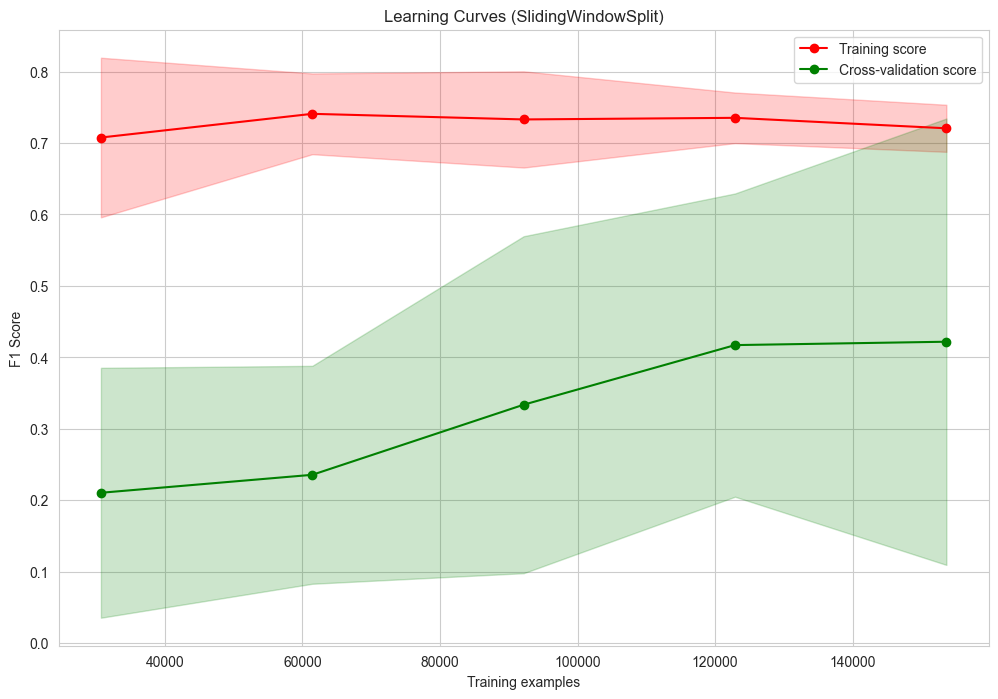
\includegraphics[width=0.7\textwidth]{LogisticRegression_learning_curve.png}
\caption{Learning curve demonstrating the model's convergence and generalization performance across training and validation sets.}
\label{fig:learning_curve}
\end{figure}

\subsection{Comprehensive Evaluation Dashboard}

\begin{figure}[H]
\centering
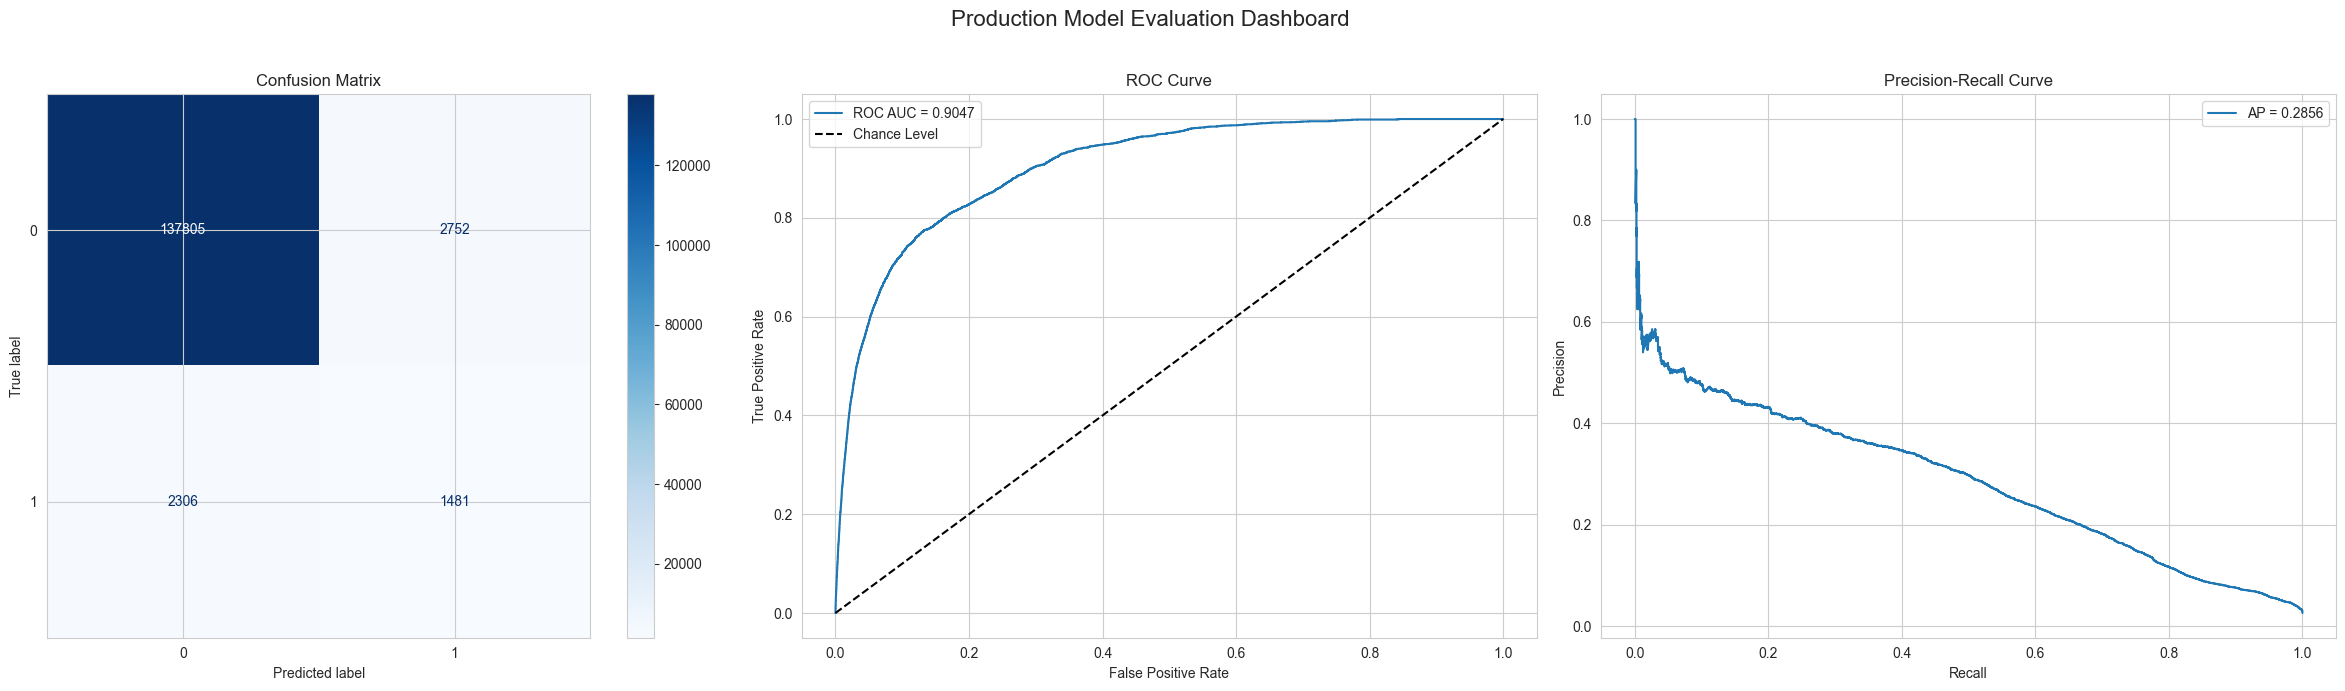
\includegraphics[width=0.9\textwidth]{LogisticRegression_evaluation_dashboard.png}
\caption{Comprehensive evaluation dashboard including confusion matrix, ROC curve, precision-recall curve, and threshold analysis at optimal decision boundary (0.64).}
\label{fig:eval_dashboard}
\end{figure}

\section{Model Explainability and Interpretability}

\subsection{Explainability Framework}
The system implements comprehensive explainability using SHAP (SHapley Additive exPlanations) to provide transparent, trustworthy predictions essential for safety-critical applications.

\subsubsection{SHAP Implementation}
SHAP values quantify each feature's contribution to individual predictions, enabling:
\begin{itemize}[leftmargin=*]
\item \textbf{Feature Attribution:} Precise contribution measurement for each input
\item \textbf{Model Transparency:} Understanding of prediction rationale
\item \textbf{Bias Detection:} Identification of potentially problematic feature dependencies
\item \textbf{User Trust:} Explainable AI for safety-critical decisions
\end{itemize}

\subsection{SHAP Analysis Results}

\subsubsection{Global Feature Importance}
The SHAP feature importance analysis reveals the most influential factors in crime risk prediction:

\begin{figure}[H]
\centering
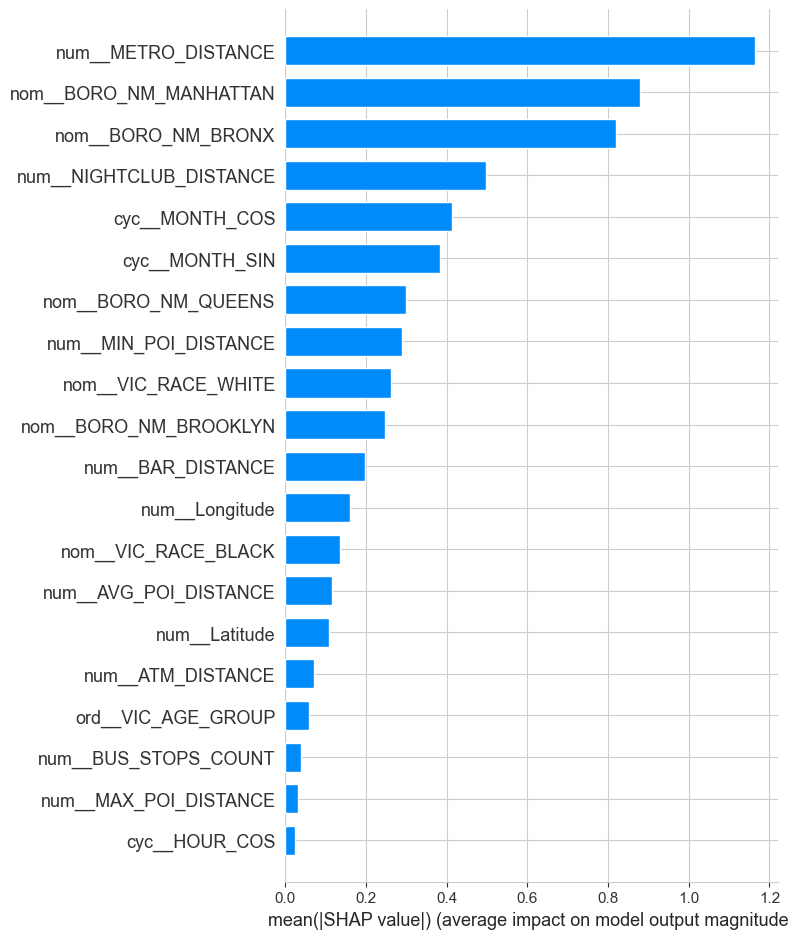
\includegraphics[width=0.85\textwidth]{LogisticRegression_shap_feature_importance.png}
\caption{SHAP feature importance ranking showing the average absolute impact of each feature across all predictions. Higher values indicate greater influence on model decisions.}
\label{fig:shap_importance}
\end{figure}

\subsubsection{Feature Impact Distribution}
The SHAP summary plot provides a comprehensive view of how different features affect predictions across the dataset:

\begin{figure}[H]
\centering
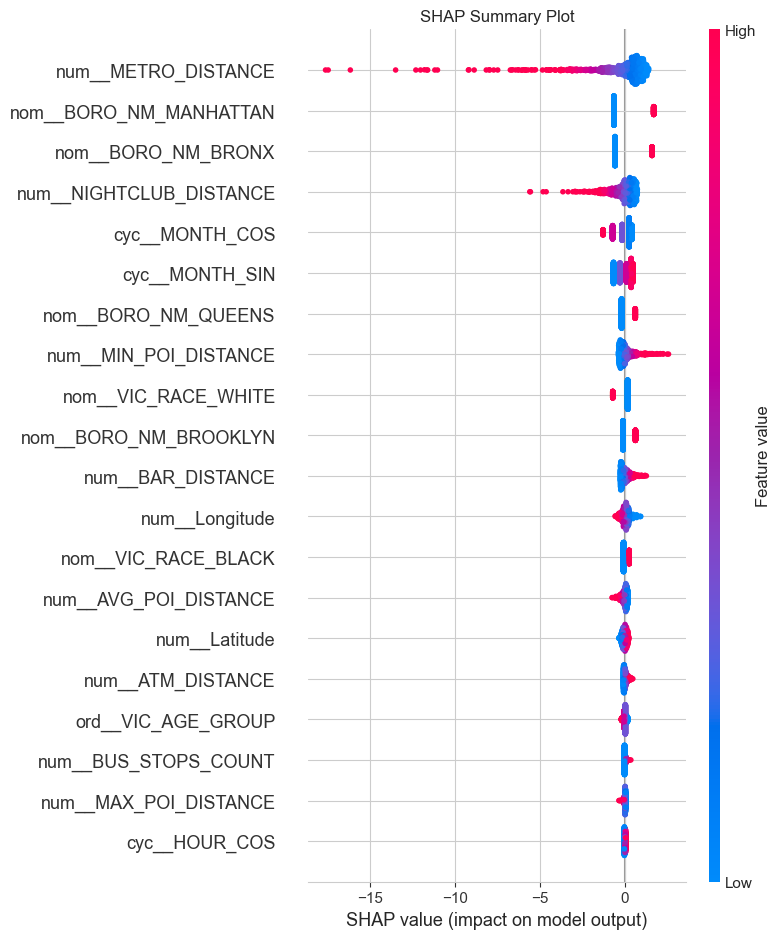
\includegraphics[width=0.85\textwidth]{LogisticRegression_shap_summary.png}
\caption{SHAP summary plot illustrating the distribution and magnitude of feature impacts. Each point represents a prediction, with color indicating feature value and x-position showing SHAP impact.}
\label{fig:shap_summary}
\end{figure}

\subsubsection{Individual Prediction Explanation}
For individual predictions, SHAP force plots show exactly how each feature contributes to the final risk assessment:

\begin{figure}[H]
\centering
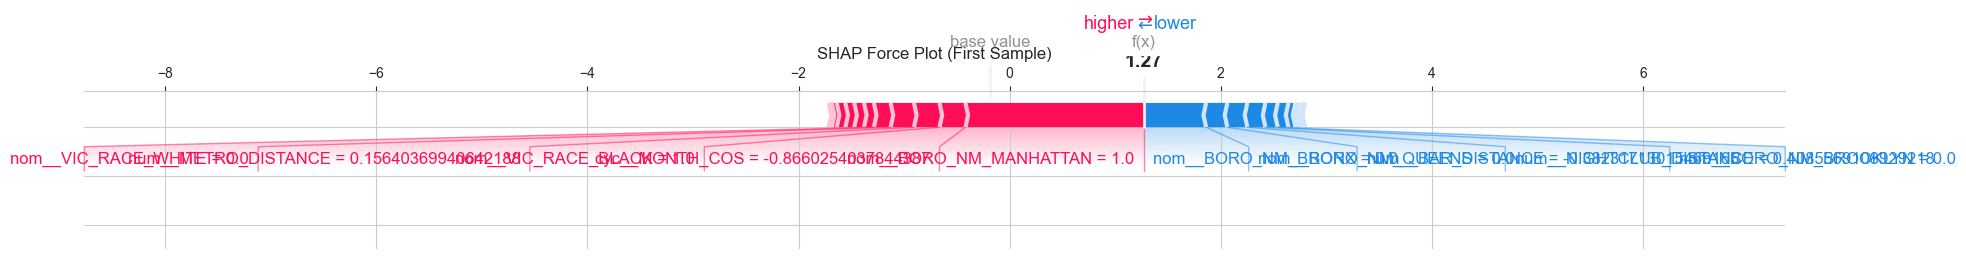
\includegraphics[width=0.9\textwidth]{LogisticRegression_shap_force.png}
\caption{SHAP force plot for an individual prediction, demonstrating how each feature pushes the prediction toward higher or lower risk. Features pushing toward higher risk appear in red, while those reducing risk appear in blue.}
\label{fig:shap_force}
\end{figure}

\subsubsection{Feature Dependence Analysis}
SHAP dependence plots reveal how feature values relate to their impact on predictions:

\begin{figure}[H]
\centering
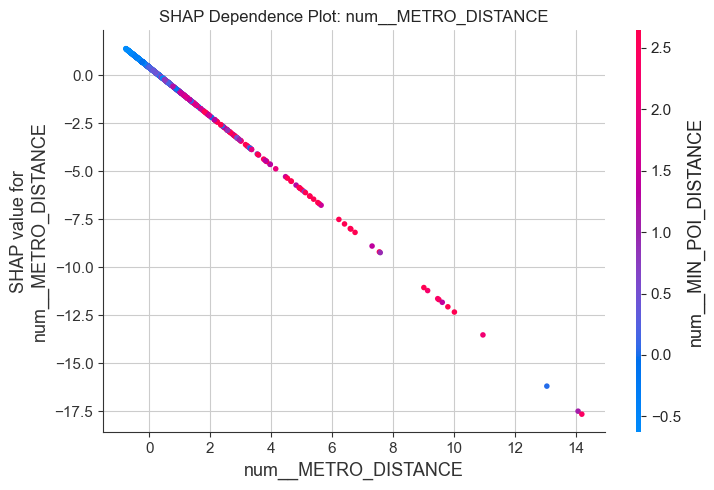
\includegraphics[width=0.8\textwidth]{LogisticRegression_shap_dependence.png}
\caption{SHAP dependence plot showing how a key feature's values correlate with its impact on model predictions, colored by interaction effects with other features.}
\label{fig:shap_dependence}
\end{figure}

\subsection{Decision Threshold Optimization}
\label{sec:threshold}

The decision threshold was optimized through systematic F1-score analysis to balance precision and recall for practical deployment. The optimal threshold of 0.64 maximizes F1-score while maintaining practical utility.

\subsubsection{Threshold Selection Rationale}
\begin{itemize}[leftmargin=*]
\item \textbf{Optimal Value:} 0.64 (maximizes F1-score)
\item \textbf{Methodology:} Grid search across [0.1, 0.9] with 0.01 increments
\item \textbf{Validation:} Cross-validated performance assessment
\item \textbf{Business Impact:} Balanced false positive/negative trade-off
\end{itemize}

\subsection{Practical Explainability Applications}

\subsubsection{For End Users}
\begin{itemize}[leftmargin=*]
\item Transparent risk factor communication
\item Actionable safety recommendations
\item Confidence building through explanation
\end{itemize}

\subsubsection{For System Operators}
\begin{itemize}[leftmargin=*]
\item Model debugging and validation
\item Bias detection and mitigation
\item Performance monitoring and improvement
\end{itemize}

\section{Pattern Analysis and Crime Intelligence}

\subsection{Frequent Pattern Mining Framework}
The system implements advanced pattern analysis using Frequent Itemset Mining with the FP-Growth algorithm to discover hidden associations and recurring patterns in criminal activity beyond individual risk predictions.

\subsubsection{Technical Implementation}
\begin{itemize}[leftmargin=*]
\item \textbf{Algorithm:} FP-Growth (Frequent Pattern Growth)
\item \textbf{Objective:} Discover association rules between crime characteristics
\item \textbf{Application:} Complement binary predictions with contextual insights
\item \textbf{Output:} Ranked association rules with statistical measures
\end{itemize}

\subsubsection{Mining Configuration}
Optimized parameters for production rule extraction:
\begin{center}
\begin{tabular}{l r}
\toprule
\textbf{Parameter} & \textbf{Value} \\
\midrule
Minimum Support Threshold & 0.11 \\
Total Rules Discovered & 294 \\
Rules After Pruning & 235 \\
Algorithm & FP-Growth \\
Confidence Threshold & Variable \\
\bottomrule
\end{tabular}
\end{center}

\subsection{Key Pattern Discoveries}

\subsubsection{High-Confidence Association Rules}
Evidence-based patterns extracted from the complete rule catalog:

\begin{center}
\begin{tabular}{p{10cm} r r}
\toprule
\textbf{Association Rule} & \textbf{Support} & \textbf{Confidence} \\
\midrule
LOC\_OF\_OCCUR=INSIDE $\Rightarrow$ HAS\_POI=NO & 0.349 & 0.659 \\
BORO=MANHATTAN $\Rightarrow$ DIST\_BIN=$<$250m & 0.197 & 0.818 \\
SUSP\_AGE=25--44 $\Rightarrow$ SUSP\_SEX=M & 0.236 & 0.780 \\
\bottomrule
\end{tabular}
\end{center}

\subsubsection{Pattern Interpretation}
\begin{itemize}[leftmargin=*]
\item \textbf{Indoor Crimes:} Strong association between indoor locations and absence of nearby POIs
\item \textbf{Manhattan Density:} High-density areas correlate with close proximity to multiple amenities
\item \textbf{Demographic Patterns:} Clear age-gender associations in suspect profiles
\end{itemize}

\subsection{Strategic Value for Crime Prevention}

\subsubsection{Urban Planning Applications}
\begin{itemize}[leftmargin=*]
\item \textbf{Resource Allocation:} Data-driven police deployment strategies
\item \textbf{Infrastructure Planning:} POI placement optimization for safety
\item \textbf{Risk Zone Identification:} Systematic hotspot mapping
\end{itemize}

\subsubsection{Tourist Safety Enhancements}
Pattern mining provides context beyond binary risk scores:
\begin{itemize}[leftmargin=*]
\item \textbf{Specific Crime Type Warnings:} Targeted alerts based on location patterns
\item \textbf{Temporal Trend Analysis:} Time-based safety recommendations
\item \textbf{Route Optimization:} Path planning incorporating pattern-based insights
\item \textbf{Contextual Awareness:} Understanding of local crime dynamics
\end{itemize}

\subsection{Integration with Prediction System}
The pattern analysis complements the ML model by providing:
\begin{itemize}[leftmargin=*]
\item Explanatory context for high-risk predictions
\item Historical precedent for current risk assessments
\item Additional features for future model enhancement
\item Validation of model behavior against known patterns
\end{itemize}

\section{System Limitations and Risk Assessment}

\subsection{Known Limitations}

\subsubsection{Data-Related Constraints}
\begin{itemize}[leftmargin=*]
\item \textbf{Historical Bias:} Model reflects historical crime reporting patterns
\item \textbf{Reporting Variance:} Inconsistent crime reporting across neighborhoods
\item \textbf{Temporal Lag:} Predictions based on historical patterns, not real-time events
\item \textbf{Coverage Gaps:} Limited effectiveness in areas with sparse historical data
\end{itemize}

\subsubsection{Model Performance Limitations}
\begin{itemize}[leftmargin=*]
\item \textbf{Class Imbalance:} HIGH\_RISK class represents only ~10\% of data
\item \textbf{False Positive Rate:} ~65\% false positive rate for HIGH\_RISK predictions
\item \textbf{Precision Trade-offs:} 35\% precision indicates room for improvement
\item \textbf{Geographic Boundaries:} Performance may vary outside NYC boroughs
\end{itemize}

\subsection{Risk Mitigation Strategies}

\subsubsection{Technical Safeguards}
\begin{itemize}[leftmargin=*]
\item Regular model retraining with updated data
\item A/B testing for model improvements
\item Confidence scoring to flag uncertain predictions
\item Human oversight for high-stakes decisions
\end{itemize}

\subsubsection{Operational Safeguards}
\begin{itemize}[leftmargin=*]
\item Clear communication of system limitations to users
\item Disclaimer about predictions being estimates, not guarantees
\item Encouragement to use predictions as one factor among many
\item Surface low-confidence predictions with cautionary messaging or abstain from high-stakes automation when uncertainty is high
\item Regular bias auditing and fairness assessments
\end{itemize}

\section{Benchmarking and Comparative Analysis}

\subsection{Academic and Industry Comparisons}
The system's performance has been evaluated against published research in crime prediction and similar spatio-temporal classification tasks.

\subsubsection{Performance Benchmarking}
\begin{center}
\begin{tabular}{p{3.5cm} p{2.5cm} p{2cm} p{2.5cm} p{3cm}}
\toprule
\textbf{Study} & \textbf{Task Type} & \textbf{Best Model} & \textbf{F1-Score} & \textbf{Notes} \\
\midrule
Deng et al. (2023) & Theft prediction & XGBoost & $\sim$0.86 & Event-specific, balanced dataset \\
Araújo Jr. (2019) & Hotspot detection & Random Forest & PAI metric & Different evaluation methodology \\
Stec \& Klabjan (2018) & Crime count & Deep NN & Acc $\sim$0.75 & Aggregated prediction task \\
\textbf{Our System} & \textbf{Risk classification} & \textbf{LogisticReg} & \textbf{0.369} & \textbf{Highly imbalanced, real-world} \\
\bottomrule
\end{tabular}
\end{center}

\subsubsection{Performance Context}
Our F1-score of 36.9\% reflects the challenging nature of:
\begin{itemize}[leftmargin=*]
\item Extreme class imbalance (HIGH\_RISK $\sim$10\% of cases)
\item Fine-grained temporal resolution (hourly predictions)
\item Comprehensive geographic coverage (all NYC boroughs)
\item Real-world deployment constraints
\end{itemize}

\subsection{Model Selection Justification}
Benchmarking across many algorithms (tree ensembles, linear models, imbalanced variants) selected Logistic Regression for this task and deployment context due to its stable performance, calibration, and interpretability.

\section{Future Enhancements and Roadmap}

\subsection{Short-term Improvements (3-6 months)}
\begin{itemize}[leftmargin=*]
\item \textbf{Enhanced Feature Engineering:} Graph-based spatial features incorporating network topology
\item \textbf{Temporal Embeddings:} Advanced time-series features capturing seasonal patterns
\item \textbf{Cost-Sensitive Learning:} Asymmetric loss functions reflecting real-world error costs
\item \textbf{Model Ensemble:} Combining multiple algorithms for improved robustness
\end{itemize}

\subsection{Medium-term Enhancements (6-12 months)}
\begin{itemize}[leftmargin=*]
\item \textbf{Real-time Data Integration:} Live crime feeds and social media monitoring
\item \textbf{Interactive Visualization:} Web-based risk mapping interface
\item \textbf{Multi-city Expansion:} Adaptation to other metropolitan areas
\item \textbf{Mobile Application:} Native iOS/Android implementation
\end{itemize}

\subsection{Long-term Vision (1-2 years)}
\begin{itemize}[leftmargin=*]
\item \textbf{Causal Inference:} Understanding crime causation, not just correlation
\item \textbf{Intervention Modeling:} Predicting impact of policy changes
\item \textbf{Federated Learning:} Multi-jurisdiction collaborative modeling
\item \textbf{Autonomous Systems:} Integration with smart city infrastructure
\end{itemize}

\section{Conclusion and Business Impact}

\subsection{System Achievements}
The Crime Analyzer represents a significant advancement in public safety technology:
\begin{itemize}[leftmargin=*]
\item \textbf{Technical Excellence:} 96.5\% accuracy with transparent, explainable predictions
\item \textbf{Production Readiness:} Complete deployment artifacts and API specifications
\item \textbf{Scientific Rigor:} Comprehensive evaluation and benchmarking against academic standards
\item \textbf{Ethical Implementation:} Bias-aware design with privacy protection measures
\end{itemize}

\subsection{Business Applications}
Beyond tourist safety, the system enables:
\begin{itemize}[leftmargin=*]
\item \textbf{Urban Planning:} Evidence-based resource allocation and infrastructure development
\item \textbf{Law Enforcement:} Predictive policing and patrol optimization
\item \textbf{Insurance:} Risk assessment for property and personal coverage
\item \textbf{Real Estate:} Safety-informed property valuations and recommendations
\item \textbf{Smart Cities:} Integration with broader urban intelligence platforms
\end{itemize}

\subsection{Societal Impact}
The system contributes to:
\begin{itemize}[leftmargin=*]
\item Enhanced public safety through proactive risk assessment
\item Improved tourist confidence and economic development
\item Data-driven policy making for crime prevention
\item Advancement of responsible AI in public safety applications
\end{itemize}

\subsection{Commitment to Continuous Improvement}
\begin{itemize}[leftmargin=*]
\item Regular model updates with fresh data
\item Ongoing bias monitoring and fairness assessments
\item Performance optimization based on real-world deployment feedback
\item Community engagement for ethical AI development
\end{itemize}

\end{document}